\documentclass[conference]{IEEEtran}
\IEEEoverridecommandlockouts
% Template version as of 6/27/2024

\usepackage{cite}
\usepackage{algorithmic}
\usepackage{graphicx}
\usepackage{textcomp}
\usepackage{xcolor}
\usepackage{amsmath,amsxtra,amssymb,amsthm,latexsym,amscd,amsfonts}
\usepackage[utf8]{vietnam}
\usepackage[english]{babel}
\usepackage{fancyhdr}
\usepackage{multirow}
\usepackage{booktabs} % Để kẻ bảng đẹp hơn
\usepackage{url}

\pagestyle{fancy}
\renewcommand{\headrulewidth}{0pt}
\renewcommand{\footrulewidth}{0pt}
\renewcommand{\sectionmark}[1]{\markright{\MakeUppercase{#1}}{}}

% Điều chỉnh lề theo template FJCAI
\setlength{\oddsidemargin}{0.5pt}
\addtolength{\textwidth}{-0.5cm}

\def\BibTeX{{\rm B\kern-.05em{\sc i\kern-.025em b}\kern-.08em
    T\kern-.1667em\lower.7ex\hbox{E}\kern-.125emX}}

\makeatletter
\def\ps@IEEEtitlepagestyle{%
\def\@oddhead{\hfil \small{\textit{Hội thảo khoa học Quốc gia về Trí tuệ nhân tạo (FJCAI) - Cần Thơ, 27-28/3/2026}\hfil}%
	\def\@evenhead{\hfil\small{\textit{Hội thảo khoa học quốc gia về Trí tuệ nhân tạo (FJCAI) - Cần Thơ, 27-28/3/2026}\hfil}}%
		\def\@oddfoot{\scriptsize \thepage \hfil }%
		\def\@evenfoot{\scriptsize \hfil \thepage}
	}
}
\makeatother

\fancyhf{}
\fancyhead[RE,LO]{\centering{\small{\textit{Hội thảo khoa học Quốc gia về Trí tuệ nhân tạo (FJCAI) - Cần Thơ, 27-28/3/2026}}}}

\begin{document}

\title{Ứng dụng Trí tuệ nhân tạo trong xây dựng hệ thống Học tăng cường hỗ trợ dạy và học STEM}

\author{\IEEEauthorblockN{1\textsuperscript{st} Nguyễn Hữu Lộc}
\IEEEauthorblockA{\textit{Khoa Công nghệ Thông tin} \\
\textit{Trường Đại học Sài Gòn}\\
TP. Hồ Chí Minh, Việt Nam \\
lockbkbang@gmail.com}
\and
\IEEEauthorblockN{2\textsuperscript{nd} Văn Tuấn Kiệt}
\IEEEauthorblockA{\textit{Khoa Công nghệ Thông tin} \\
\textit{Trường Đại học Sài Gòn}\\
TP. Hồ Chí Minh, Việt Nam \\
vankiet27012004@gmail.com}
}

\maketitle

\begin{abstract}
Trong kỷ nguyên công nghiệp 4.0, giáo dục STEM đóng vai trò then chốt trong việc đào tạo nguồn nhân lực chất lượng cao. Tuy nhiên, các phương pháp giảng dạy truyền thống và hệ thống quản lý học tập (LMS) hiện hành thường áp dụng cách tiếp cận ``một kích cỡ cho tất cả'', thất bại trong việc đáp ứng nhu cầu cá nhân hóa của từng người học. Bài báo này đề xuất một hệ thống gợi ý lộ trình học tập thông minh sử dụng kỹ thuật Học tăng cường (Reinforcement Learning - RL), cụ thể là thuật toán Q-learning, được tích hợp vào nền tảng Moodle qua chuẩn LTI 1.3. Hệ thống mô hình hóa quá trình học tập dưới dạng Quy trình quyết định Markov (MDP), sử dụng dữ liệu hành vi thực tế để phân cụm người học và tối ưu hóa chiến lược gợi ý. Kết quả thực nghiệm mô phỏng trên 500 vòng lặp cho thấy thuật toán giúp tăng 22.5\% điểm số trung bình và giảm 51.0\% số lượng kỹ năng yếu so với phương pháp truyền thống.
\end{abstract}

\begin{IEEEkeywords}
Học tăng cường, Q-learning, Cá nhân hóa học tập, Giáo dục STEM, Data-driven Simulation, MDP
\end{IEEEkeywords}

\section{Giới thiệu}
\label{sec:intro}
Sự phát triển mạnh mẽ của Trí tuệ nhân tạo (AI) đang định hình lại nhiều lĩnh vực, trong đó có giáo dục. Theo nghiên cứu của Frey và Osborne, khoảng 47\% các công việc truyền thống có nguy cơ bị tự động hóa, đặt ra yêu cầu cấp thiết về việc trang bị các kỹ năng mới cho người lao động, đặc biệt là các kỹ năng STEM (Khoa học, Công nghệ, Kỹ thuật và Toán học)\cite{b2}. Giáo dục STEM chú trọng phát triển tư duy phản biện và khả năng giải quyết vấn đề, tuy nhiên, việc triển khai hiệu quả gặp nhiều rào cản do sự đa dạng về năng lực và tốc độ tiếp thu của học viên.

Thách thức lớn nhất hiện nay là cá nhân hóa trải nghiệm học tập (Personalized Adaptive Learning - PAL) trên quy mô lớn. Các hệ thống LMS truyền thống như Moodle, Blackboard chủ yếu đóng vai trò lưu trữ tài liệu và quản lý điểm số, thiếu khả năng phân tích hành vi để đưa ra các can thiệp sư phạm kịp thời\cite{b1}. Tại Việt Nam, các nghiên cứu về ứng dụng AI trong giáo dục chủ yếu tập trung vào bài toán dự báo (prediction) - ví dụ như dự báo nguy cơ bỏ học hoặc dự đoán điểm số cuối kỳ - mà chưa chú trọng nhiều đến bài toán đưa ra khuyến nghị hành động (prescription) để cải thiện kết quả đó\cite{b4}.

Để giải quyết vấn đề này, nhu cầu về một hệ thống hỗ trợ dạy và học STEM cá nhân hóa ứng dụng Học tăng cường (Reinforcement Learning - RL) trở nên cấp thiết. RL cho phép hệ thống tự động tối ưu hóa chiến lược giảng dạy thông qua cơ chế thử-sai (trial-and-error).

Nghiên cứu này đóng góp vào lĩnh vực Cá nhân hóa học tập (Personalized Adaptive Learning) thông qua ba điểm chính:
\begin{enumerate}
    \item \textbf{Đề xuất khung giải pháp thích ứng:} Xây dựng mô hình Quy trình quyết định Markov (MDP) với hàm phần thưởng đa mục tiêu, kết hợp giữa đặc điểm phân cụm người học và lý thuyết hành vi (ICAP framework).
    \item \textbf{Quy trình Mô phỏng hướng dữ liệu (Data-driven Simulation):} Giải quyết thách thức ``khởi động lạnh'' (cold-start) và sự khan hiếm dữ liệu thực nghiệm bằng cách xây dựng môi trường giả lập dựa trên tham số thống kê từ dữ liệu khóa học thực tế.
    \item \textbf{Kiểm chứng thực nghiệm:} Chứng minh hiệu quả của thuật toán Q-learning thông qua A/B testing trên tập dữ liệu mô phỏng, cho thấy sự vượt trội so với các chiến lược truyền thống về điểm số và mức độ tham gia.
\end{enumerate}

\begin{figure}[htbp]
\centerline{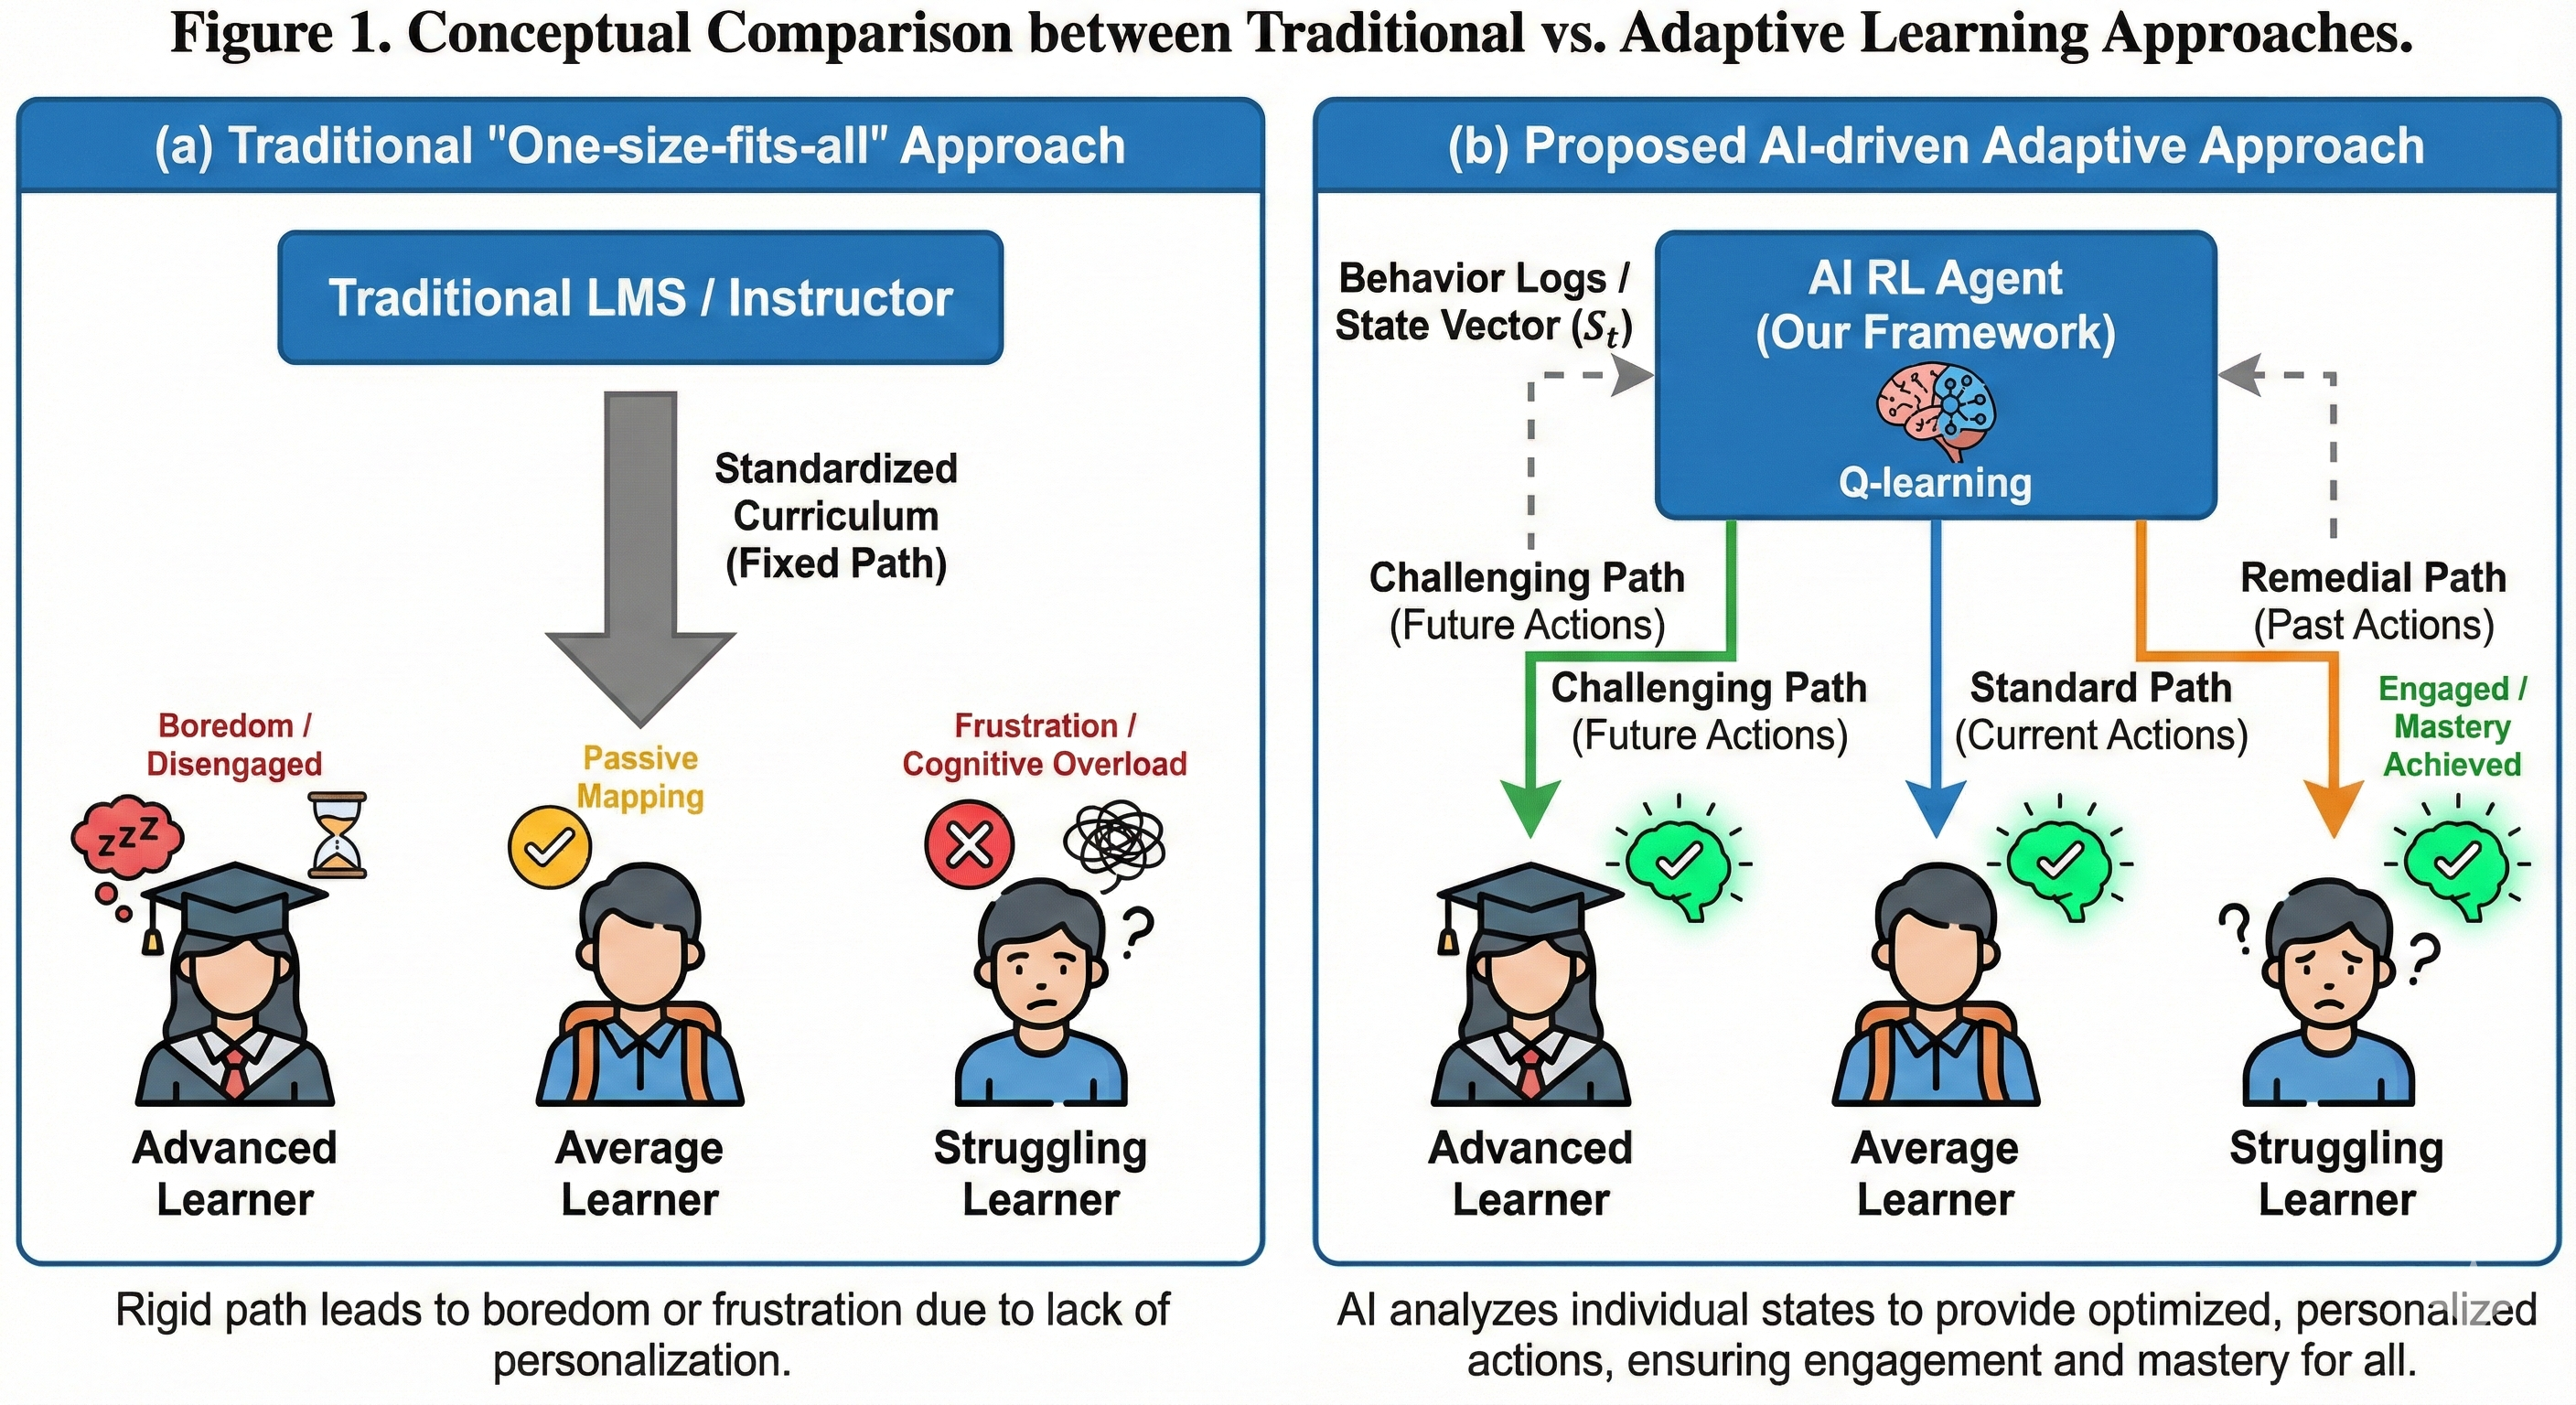
\includegraphics[width=\linewidth]{fig1_problem_concept.png}} % Đặt tên file ảnh là fig1_problem_concept.png
\caption{Comparison of learning approaches. (a) The traditional approach applies a fixed curriculum to divergent learners, leading to suboptimal engagement outcomes like boredom or frustration. (b) The proposed framework utilizes an AI Reinforcement Learning Agent to analyze individual student states from log data and recommend personalized actions (remedial, standard, or challenging), aiming for maximized engagement and mastery for all learner types.}
\label{fig:concept}
\end{figure}

\section{Phương pháp Đề xuất}
\label{sec:methodology}

Dựa trên các hạn chế của LMS truyền thống, nghiên cứu đề xuất một khung giải pháp học tập thích ứng (Adaptive Learning Framework) sử dụng thuật toán Q-learning. Quy trình xử lý tổng thể đi từ dữ liệu hành vi thô, qua bước trích xuất đặc trưng để xây dựng không gian trạng thái, và cuối cùng là tác nhân AI đưa ra quyết định tối ưu (Hình \ref{fig:proposed_method}).

% Hình 2: Tổng quan phương pháp (Overview)
\begin{figure}[htbp]
\centerline{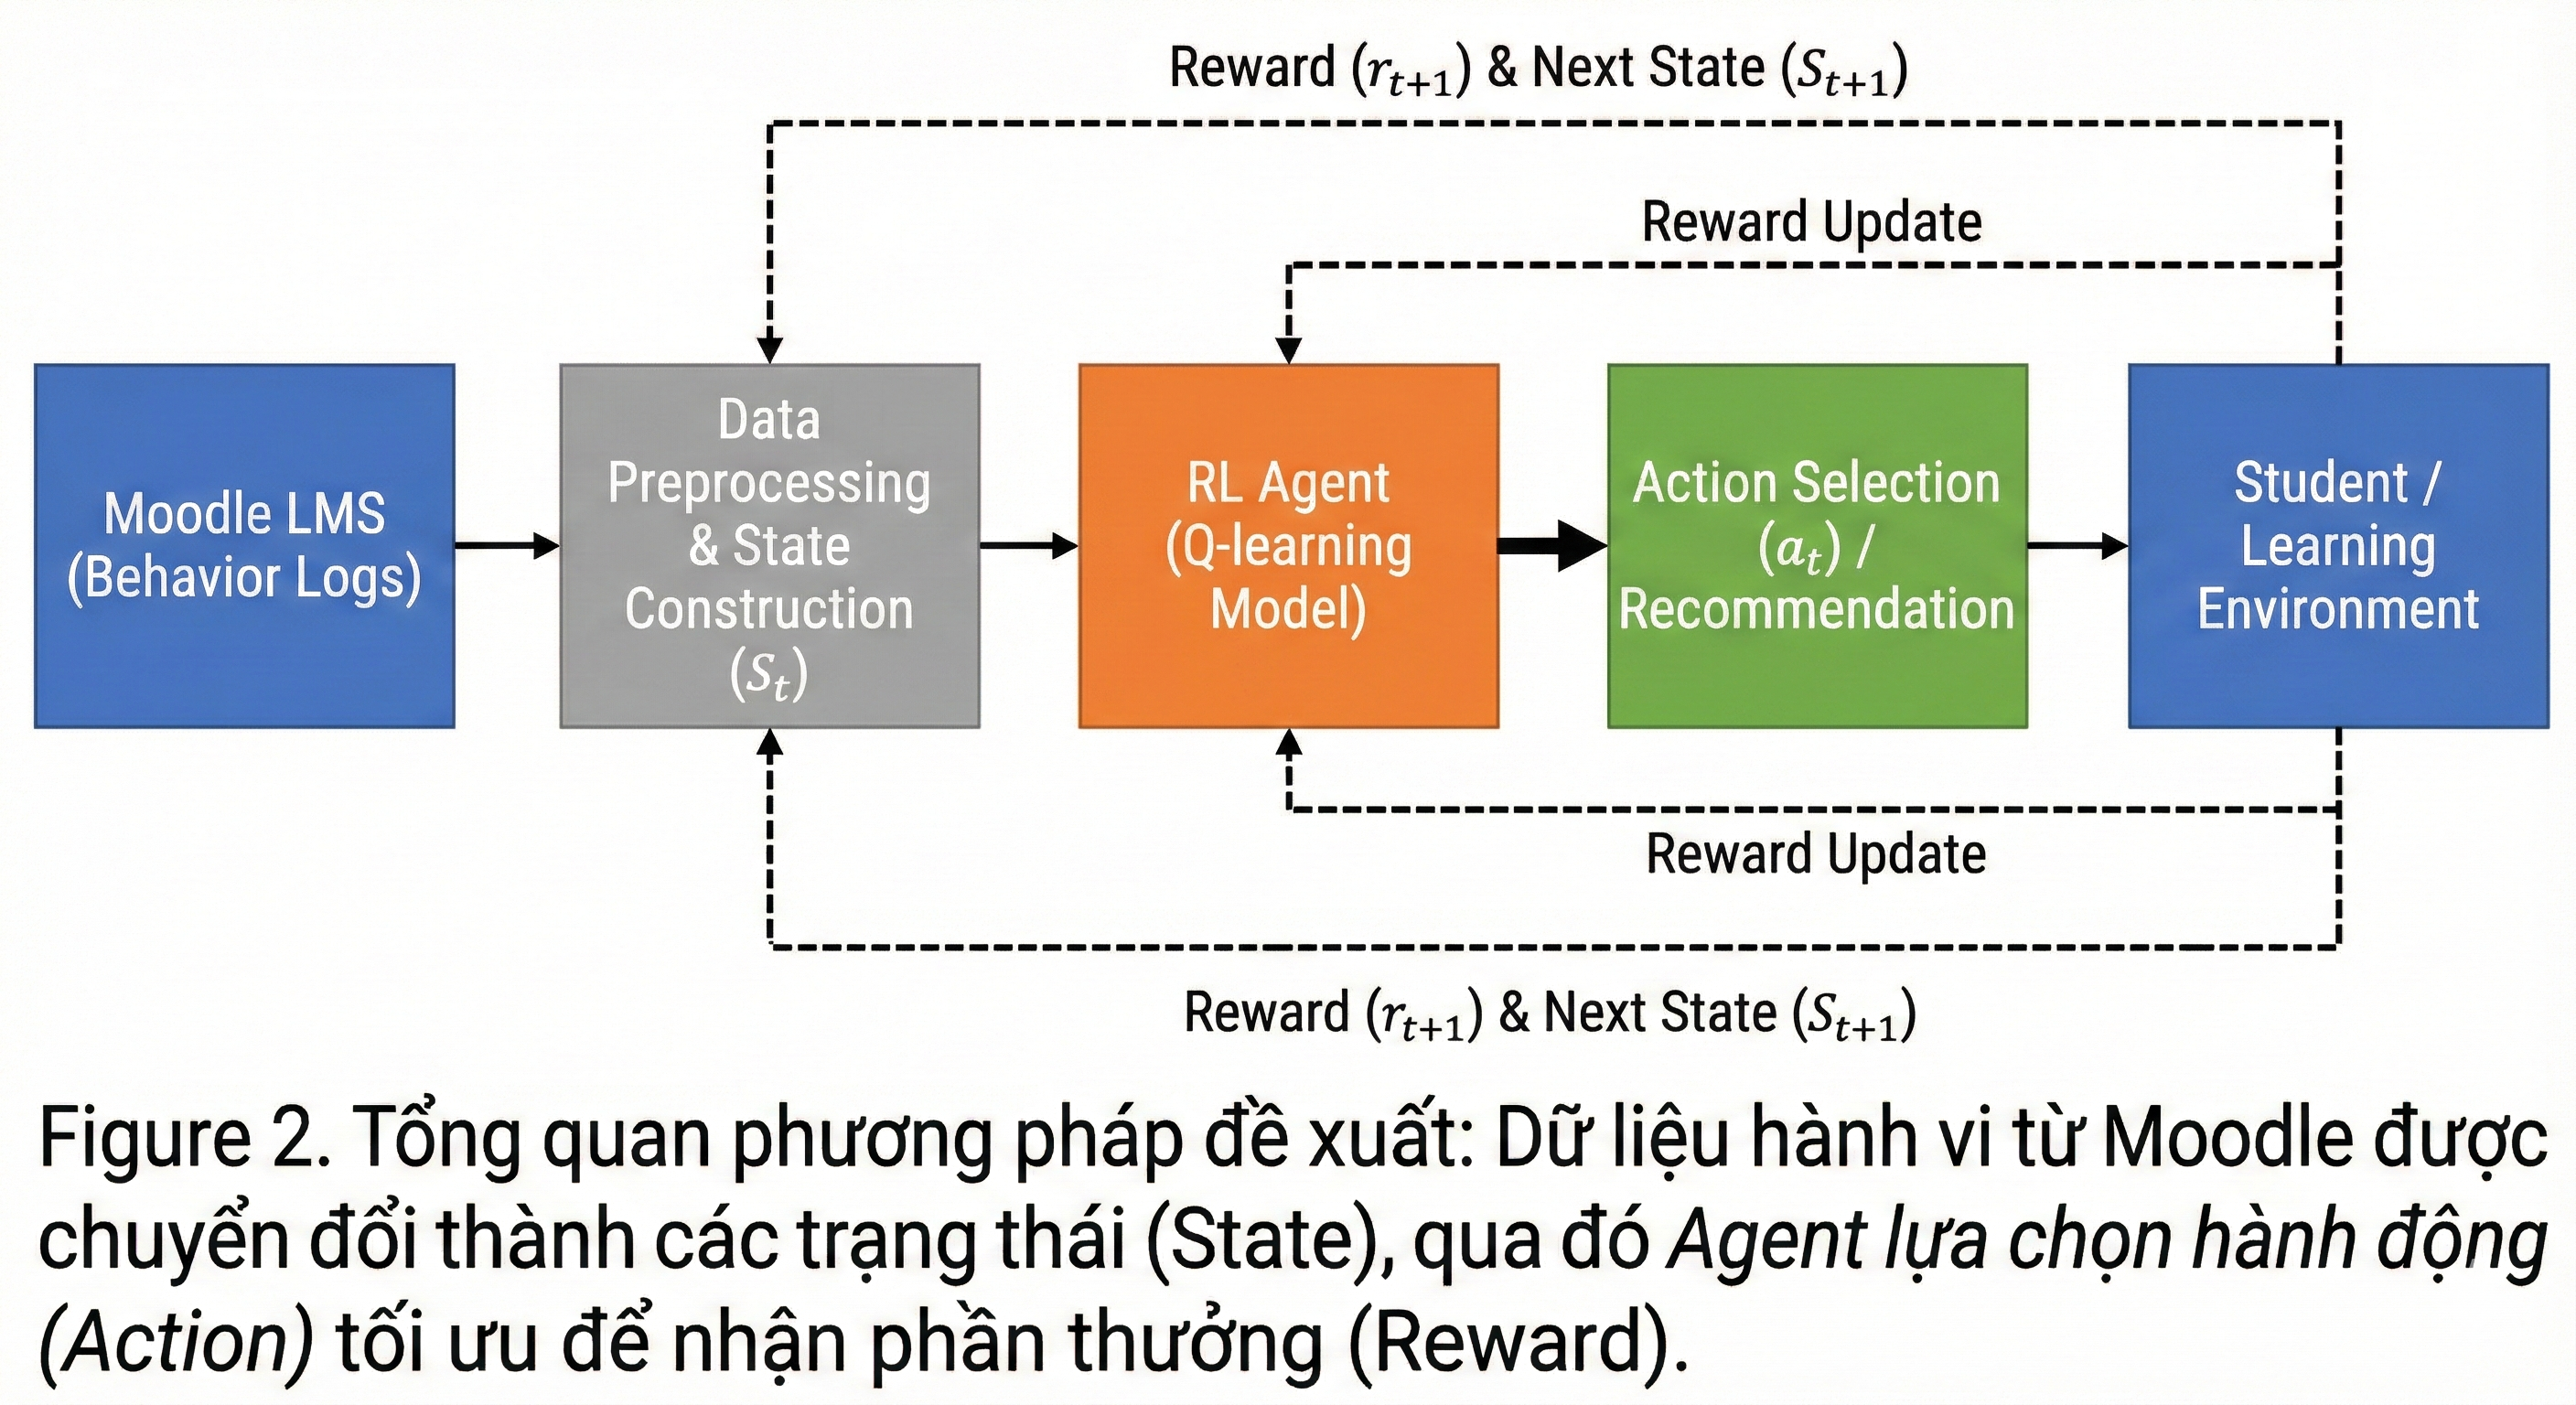
\includegraphics[width=\linewidth]{fig2_method_overview.png}}
\caption{Tổng quan phương pháp đề xuất: Dữ liệu hành vi từ Moodle được chuyển đổi thành các trạng thái (State), qua đó Agent lựa chọn hành động (Action) tối ưu để nhận phần thưởng (Reward).}
\label{fig:proposed_method}
\end{figure}

\subsection{Mô hình hóa bài toán (Problem Formulation)}
Để cá nhân hóa lộ trình học tập, chúng tôi mô hình hóa bài toán dưới dạng Quy trình Quyết định Markov (MDP), được định nghĩa bởi bộ ba $<S, A, R>$ như sau:

\subsubsection{Không gian Trạng thái (State Space - $S$)}
Tại thời điểm $t$, hệ thống quan sát trạng thái người học $S_t$. Để đảm bảo tính tổng quát, $S_t$ được định nghĩa là một vector đặc trưng $d$ chiều:
\begin{equation}
S_t = \{f_1, f_2, ..., f_d\}
\end{equation}
Trong nghiên cứu này, chúng tôi đề xuất bộ đặc trưng bao gồm: 
\begin{itemize}
    \item $C$ (Cluster): Nhóm người học xác định qua phân cụm.
    \item $M$ (Module): Chỉ số bài học hiện tại.
    \item $P$ (Progress): Mức độ hoàn thành module.
    \item $Sc$ (Score): Phân loại điểm số tích lũy.
    \item $Ph$ (Phase): Giai đoạn học tập (ví dụ: theo khung ICAP).
    \item $E$ (Engagement): Mức độ tương tác.
\end{itemize}

\subsubsection{Không gian Hành động (Action Space - $A$)}
Dựa trên $S_t$, tác nhân (Agent) lựa chọn một hành động $a_t$ từ tập hợp $A$ gồm $m$ hành động sư phạm khả dĩ ($A = \{a_0, a_1, ..., a_{m-1}\}$). Các hành động này được phân loại theo trục thời gian (Quá khứ - Hiện tại - Tương lai) nhằm phục vụ các chiến lược ôn tập (Remedial) hoặc bồi dưỡng (Advanced).

\subsubsection{Hàm phần thưởng (Reward Function - $R$)}
Mục tiêu của hệ thống là tối đa hóa tổng phần thưởng tích lũy. Hàm thưởng được thiết kế đa mục tiêu:
\begin{equation}
R_{total} = R_{base} + R_{LO} + R_{bonus} - P_{penalty}
\end{equation}
Trong đó, $R_{base}$ là phần thưởng cơ bản, $R_{LO}$ dựa trên mức độ đạt chuẩn đầu ra, $R_{bonus}$ cho các chuỗi hành vi tốt, và $P_{penalty}$ là điểm phạt để hạn chế hành vi kém hiệu quả.

\subsection{Quy trình Xử lý dữ liệu và Phân cụm}
Dữ liệu log thô từ LMS thường chứa nhiễu và không cấu trúc. Trước khi đưa vào mô hình RL, dữ liệu cần được tiền xử lý và chuẩn hóa. Thuật toán K-means được áp dụng để phân chia người học thành $K$ cụm (Clusters) có đặc điểm hành vi tương đồng. Việc xác định giá trị $K$ tối ưu được thực hiện thông qua phương pháp Elbow và chỉ số Silhouette. Giá trị Cluster ID sau đó trở thành một thành phần quan trọng trong vector trạng thái $S_t$.

\subsection{Thuật toán Q-learning}
Hệ thống sử dụng thuật toán Q-learning để cập nhật bảng giá trị Q (Q-table) theo công thức Bellman:
\begin{equation}
Q(s, a) \leftarrow Q(s, a) + \alpha [r + \gamma \max_{a'} Q(s', a') - Q(s, a)]
\end{equation}
Trong đó $\alpha$ là tốc độ học và $\gamma$ là hệ số chiết khấu. Chiến lược $\epsilon$-greedy được áp dụng để cân bằng giữa khám phá (Exploration) và khai thác (Exploitation).

\begin{figure}[htbp]
\centerline{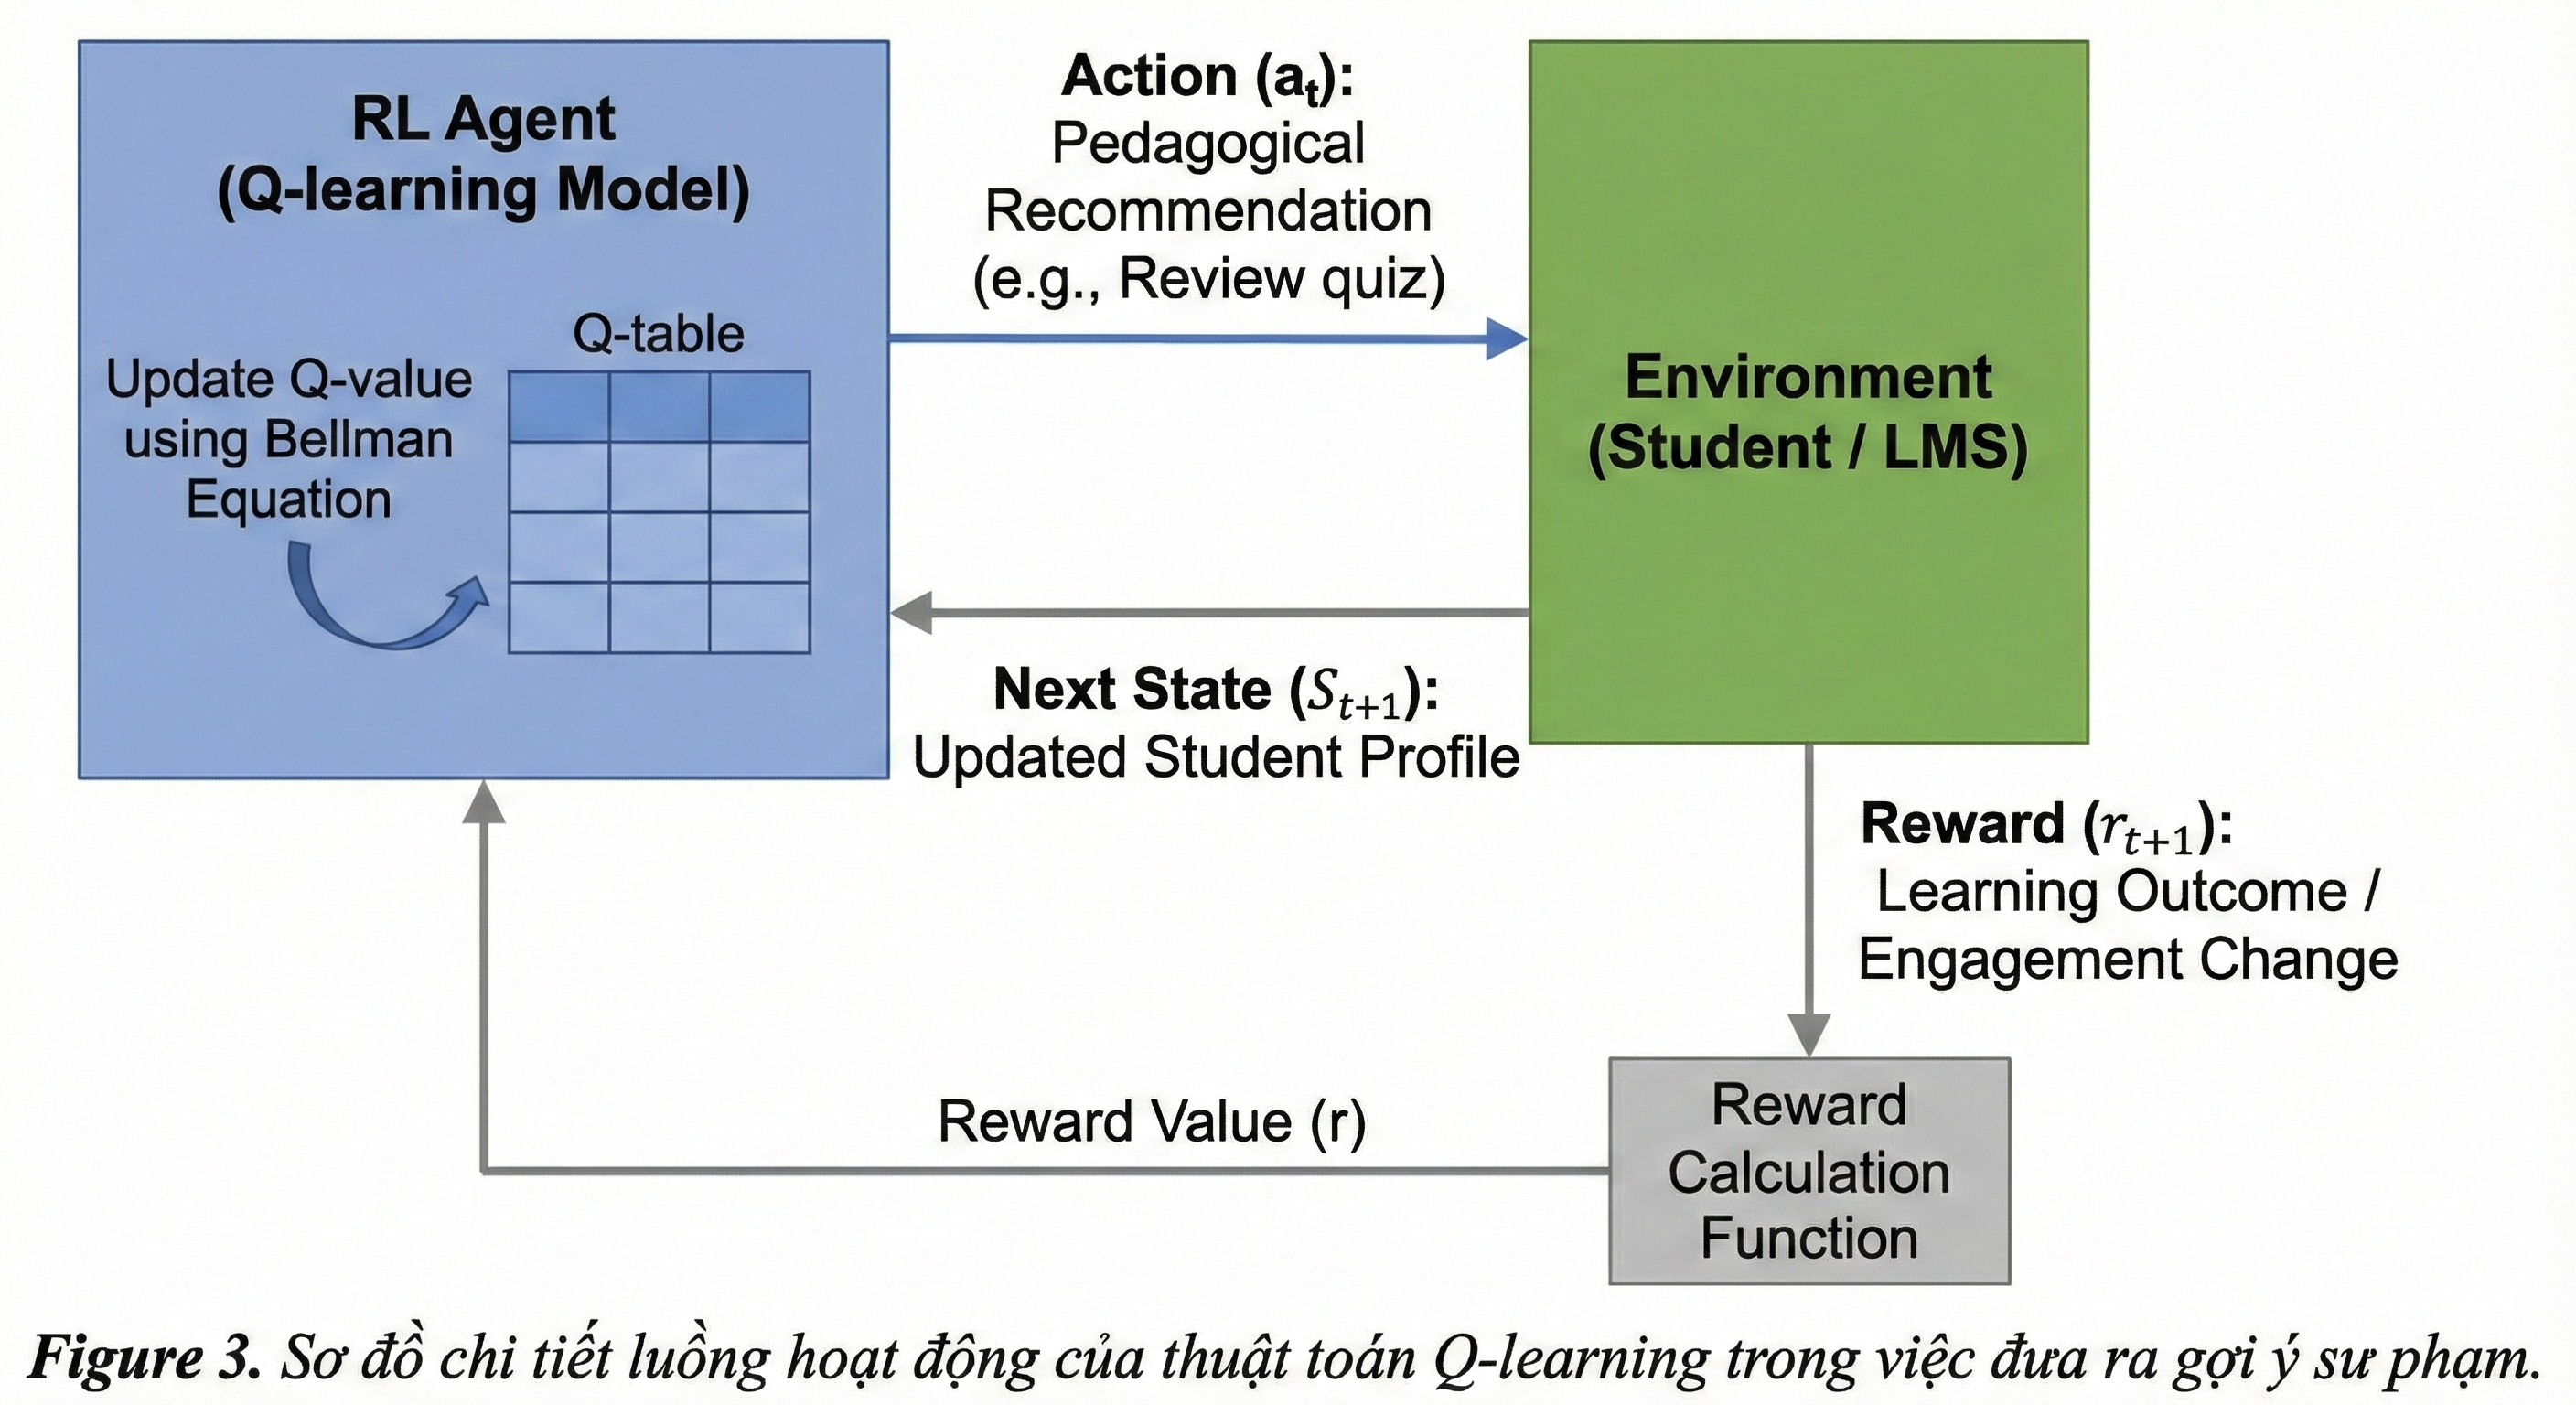
\includegraphics[width=0.9\linewidth]{fig3_qlearning_diagram.png}} 
\caption{Sơ đồ chi tiết luồng hoạt động của thuật toán Q-learning trong việc đưa ra gợi ý sư phạm.}
\label{fig:qlearning_diagram}
\end{figure}

\subsection{Khung giải thích mô hình (Explainability Framework)}
Để giải quyết tính "hộp đen" của bảng Q-table và tăng sự tin cậy sư phạm, nghiên cứu tích hợp phương pháp \textbf{SHAP (SHapley Additive exPlanations)}~\cite{shap_arxiv}.

\subsubsection{Cơ sở toán học}
Giá trị SHAP $\phi_i$ đo lường đóng góp biên của đặc trưng $i$ vào giá trị Q dự đoán, dựa trên lý thuyết trò chơi hợp tác:
\begin{equation}
\phi_i = \sum_{S \subseteq F \setminus \{i\}} \frac{|S|!(|F|-|S|-1)!}{|F|!} [f(S \cup \{i\}) - f(S)]
\end{equation}
trong đó $F$ là tập hợp đặc trưng và $f$ là hàm tra cứu Q-table. Tính chất cộng tính giúp phân rã giá trị Q thành tổng các đóng góp: $Q(s, a^*) = \phi_0 + \sum \phi_i(s)$.

\subsubsection{Cơ chế triển khai}
Do không gian trạng thái rời rạc, chúng tôi sử dụng \textbf{KernelExplainer} để xấp xỉ giá trị Shapley. Quy trình bao gồm: (1) Xây dựng hàm dự đoán từ Q-table đã hội tụ; (2) Lấy mẫu nền (Background sampling) từ tập trạng thái quan sát được; và (3) Tính toán trọng số đóng góp cho từng đặc trưng trong vector trạng thái $S_t$.

\subsection{Khung mô phỏng hướng dữ liệu (Data-driven Simulation Framework)}
Để giải quyết bài toán "khởi động lạnh" (Cold-start) và đảm bảo tính hội tụ của thuật toán trước khi triển khai thực tế, chúng tôi đề xuất quy trình huấn luyện hai giai đoạn dựa trên khái niệm "Digital Twin" (Bản sao số).

\subsubsection{Mô hình hóa Xác suất chuyển đổi (Transition Probability Modeling)}
Dựa trên dữ liệu lịch sử $\mathcal{D}_{history}$, hệ thống xây dựng một Ma trận xác suất chuyển đổi (Transition Probability Matrix - TPM) $\mathcal{P}$. Với mỗi cặp trạng thái - hành động $(s, a)$, xác suất người học chuyển sang trạng thái tiếp theo $s'$ được ước lượng bởi:
\begin{equation}
P(s' | s, a) = \frac{count(s, a, s')}{\sum_{s^*} count(s, a, s^*)}
\end{equation}
Ma trận $\mathcal{P}$ này đóng vai trò là "môi trường nền" (Baseline Environment), phản ánh thói quen và phản ứng tự nhiên của người học trong quá khứ.

\subsubsection{Cơ chế Huấn luyện và Đánh giá (Training \& Evaluation Pipeline)}
Quy trình được thực hiện theo chu trình khép kín:
\begin{enumerate}
    \item \textbf{Khởi tạo (Initialization):} Xây dựng các Tác nhân Người học (Student Agents) với các đặc trưng hành vi được tham số hóa từ $\mathcal{D}_{history}$.
    \item \textbf{Huấn luyện (Training):} Agent tương tác với các Tác nhân Người học trong môi trường giả lập để tối ưu bảng Q-table.
    \item \textbf{Đối sánh (Comparison):} So sánh chiến lược tối ưu $\pi^*$ của Q-learning với chiến lược ngẫu nhiên có tham số (Parametric Policy) mô phỏng lại hành vi lịch sử $\mathcal{P}$.
\end{enumerate}

\section{Thực nghiệm và Kết quả}
\label{sec:experiments}

\subsection{Thiết lập Môi trường Giả lập (Simulation Setup)}

\subsubsection{Mô hình hóa Phong cách học tập}
Các tác nhân ảo (Virtual Agents) không hành động ngẫu nhiên mà sở hữu các phong cách học tập phi tuyến tính. Phân phối phong cách được thiết lập dựa trên tham số thực tế:
\begin{itemize}
    \item \textbf{Linear Learner (70\%):} Tuân thủ lộ trình tuần tự truyền thống.
    \item \textbf{Practice-first (10\%):} Ưu tiên thực hiện bài tập/quiz trước khi xem lý thuyết.
    \item \textbf{Video/Reading-first (20\%):} Ưu tiên tiêu thụ nội dung thụ động trước khi tương tác.
\end{itemize}

\subsubsection{Tham số hành vi theo Phân cụm}
Hành vi của tác nhân được tham số hóa chi tiết dựa trên cụm (Cluster):
\begin{itemize}
    \item \textbf{Nhóm Weak:} Tốc độ học thấp ($\alpha \approx 0.22$) và độ biến động điểm số cao ($\sigma=0.18$).
    \item \textbf{Nhóm Strong:} Tốc độ học cao ($\alpha \approx 0.30$), tỷ lệ thành công cao ($0.90$) và độ biến động thấp.
\end{itemize}

\subsection{Thiết lập thực nghiệm (Experimental Setup)}

\subsubsection{Dữ liệu huấn luyện (Dataset Ground Truth)}
Nghiên cứu sử dụng bộ dữ liệu chuẩn \textit{Moodle Log \& Grades} \cite{dataset_kaggle}. Trong số các khóa học có sẵn, chúng tôi lựa chọn \textbf{Khóa học ID 670} làm cơ sở để xây dựng môi trường mô phỏng (Data-driven Environment).

Quyết định này dựa trên sự cân bằng lý tưởng của dữ liệu: Khóa học ghi nhận 13,995 điểm tương tác từ 23 sinh viên với phân phối điểm số chuẩn ($\mu=7.64, \sigma=2.95$). Điều này khắc phục được hạn chế dữ liệu bị lệch (skewed data) thường thấy ở các khóa học khác (ví dụ Course ID 42 có Mean=1.07), giúp thuật toán phân biệt rõ ràng chiến lược học tập giữa các nhóm sinh viên (Giỏi, Khá, Yếu).

\subsubsection{Tiền xử lý và Trích xuất đặc trưng}
Để giải quyết bài toán bùng nổ không gian trạng thái, chúng tôi áp dụng kỹ thuật \textbf{Lọc tương quan (Correlation Filtering)} với ngưỡng 0.95 trên 114 đặc trưng hành vi thô ban đầu. Kết quả đã thu gọn không gian đầu vào xuống còn \textbf{15 đặc trưng cốt lõi} (Hình \ref{fig:correlation}), loại bỏ hoàn toàn hiện tượng đa cộng tuyến.

\begin{figure}[htbp]
\centerline{\includegraphics[width=\columnwidth]{correlation.png}}
\caption{Ma trận tương quan Pearson giữa 15 đặc trưng hành vi cốt lõi. Các cặp biến có $|r| > 0.95$ đã được loại bỏ, đảm bảo không có đa cộng tuyến trong mô hình Q-learning.}
\label{fig:correlation}
\end{figure}

Sau bước trích xuất, thuật toán K-means được áp dụng với $K=6$ cụm. Đáng chú ý, cụm dữ liệu của giảng viên đã được phát hiện và loại bỏ khỏi tập huấn luyện để đảm bảo tính chính xác cho Agent.

\subsubsection{Tham số mô hình (Model Parameters)}
Trong quá trình thực nghiệm, các tham số mô hình được thiết lập chi tiết để đảm bảo sự hội tụ của thuật toán:

\begin{itemize}
    \item \textbf{Không gian trạng thái ($S$):} Trạng thái $S_t$ được định nghĩa là vector 6 chiều phản ánh ngữ cảnh người học:
    \begin{equation}
    S_t = (C, M, P, Sc, Ph, E)
    \end{equation}
    Trong đó: $C$ là cụm người học ($K=6$); $M$ là chỉ số module; $P, Sc$ là mức tiến độ và điểm số (rời rạc hóa 4 mức); $Ph$ là giai đoạn học tập ($0$: Pre, $1$: Active, $2$: Reflective); và $E$ là mức độ tương tác (Low, Med, High). Kích thước không gian là $5 \times 6 \times 4 \times 4 \times 3 \times 3 \approx 4,320$ trạng thái.

    \item \textbf{Không gian hành động ($A$):} Gồm $m=15$ hành động được sàng lọc qua bộ lọc ICAP và Pareto ($>1\%$ tần suất). Để tối ưu hiển thị, các hành động được nhóm theo ngữ cảnh thời gian như trình bày tại Bảng \ref{tab:action_space_compact}.

    \item \textbf{Tham số Q-learning:} Tốc độ học $\alpha=0.1$, hệ số chiết khấu $\gamma=0.95$, và chiến lược $\epsilon$-greedy giảm dần.
\end{itemize}

\begin{table}[htbp]
\caption{Không gian hành động hoàn chỉnh (15 Actions)}\label{tab:action_space_compact}
\begin{center}
\resizebox{\columnwidth}{!}{% Resize bảng để vừa khít cột báo
\begin{tabular}{ccll}
\toprule
\textbf{Nhóm} & \textbf{ID} & \textbf{Mã hành động} & \textbf{Ý nghĩa sư phạm} \\
\midrule
\multirow{5}{*}{\shortstack{PAST\\(Ôn tập)}} 
 & 0 & view\_assign\_past & Xem lại yêu cầu cũ \\
 & 1 & view\_content\_past & Ôn lại bài giảng cũ \\
 & 2 & attempt\_quiz\_past & Làm lại trắc nghiệm cũ \\
 & 3 & review\_quiz\_past & Phân tích lỗi sai cũ \\
 & 4 & post\_forum\_past & Thảo luận chủ đề cũ \\
\midrule
\multirow{7}{*}{\shortstack{CURRENT\\(Hiện tại)}} 
 & 5 & view\_assign\_curr & Xem yêu cầu bài mới \\
 & 6 & view\_content\_curr & Học nội dung tuần này \\
 & 7 & submit\_assign\_curr & Nộp bài tập lớn \\
 & 8 & attempt\_quiz\_curr & Làm bài kiểm tra \\
 & 9 & submit\_quiz\_curr & Nộp bài lấy điểm \\
 & 10 & review\_quiz\_curr & Xem kết quả vừa nộp \\
 & 11 & post\_forum\_curr & Thảo luận bài hiện tại \\
\midrule
\multirow{3}{*}{\shortstack{FUTURE\\(Chuẩn bị)}} 
 & 12 & view\_content\_fut & Xem trước bài mới \\
 & 13 & attempt\_quiz\_fut & Thử sức bài tương lai \\
 & 14 & post\_forum\_fut & Tìm hiểu chủ đề sắp tới \\
\bottomrule
\end{tabular}
}
\end{center}
\end{table}

% \subsection{Hiện thực hóa hệ thống (System Implementation)}
% Để chứng minh tính khả thi kỹ thuật, khung giải pháp đã được hiện thực hóa và triển khai thử nghiệm dưới dạng kiến trúc Microservices (Hình \ref{fig:microservice}). Hệ thống bao gồm \textit{Recommend Service} giao tiếp với Moodle LMS thông qua chuẩn LTI 1.3, sử dụng MongoDB để lưu trữ log hành vi tốc độ cao.

% \begin{figure}[htbp]
% \centerline{\includegraphics[width=0.85\linewidth]{microservice.png}}
% \caption{Kiến trúc Microservices được sử dụng để triển khai hệ thống trong thực nghiệm.}
% \label{fig:microservice}
% \end{figure}

\subsection{Độ đo đánh giá (Evaluation Metrics)}
Hiệu quả của mô hình được đánh giá qua các chỉ số:
\begin{itemize}
    \item \textbf{Tổng phần thưởng tích lũy (Total Reward):} Đo lường mức độ hội tụ của Agent.
    \item \textbf{Điểm số trung bình (Average Score):} Điểm kết thúc khóa học (thang 10).
    \item \textbf{Số kỹ năng yếu (Weak Skills Count):} Số lượng Chuẩn đầu ra (LO) có độ thông thạo $< 0.5$.
\end{itemize}

\subsection{Kết quả so sánh (A/B Testing)}
Quá trình huấn luyện diễn ra qua 500 episodes với tham số $\alpha=0.1$, $\gamma=0.95$. Kết quả định lượng tổng hợp tại Bảng \ref{tab:results} và chi tiết từng phân cụm tại Hình \ref{fig:eval_result} cho thấy sự vượt trội rõ rệt của thuật toán Q-learning.

\begin{figure}[htbp]
\centerline{\includegraphics[width=\columnwidth]{evaluate_qlearning.png}}
\caption{So sánh hiệu suất giữa Q-Learning và Param Policy trên các chỉ số: Phần thưởng (Reward), Điểm số (Score), và Độ thành thạo (LO Mastery).}
\label{fig:eval_result}
\end{figure}

\begin{table}[htbp]
\caption{Kết quả so sánh hiệu suất trung bình}\label{tab:results}
\begin{center}
\small
\begin{tabular}{p{2.8cm}ccc}
\toprule
\textbf{Chỉ số} & \textbf{Đối chứng} & \textbf{Q-learning} & \textbf{Cải thiện} \\
\midrule
Tổng phần thưởng & 88.4 & 389.6 & \textbf{+340.8\%} \\
Điểm TB (thang 10) & 6.25 & 7.66 & \textbf{+22.5\%} \\
Số kỹ năng yếu & 3.02 & 1.48 & \textbf{-51.0\%} \\
\bottomrule
\end{tabular}
\end{center}
\end{table}

\subsection{Phân tích độ quan trọng đặc trưng}
Phân tích SHAP (Hình \ref{fig:shap_distribution}) trên mô hình đã huấn luyện chỉ ra rằng \textit{Module ID} và \textit{Engagement} là hai yếu tố ảnh hưởng nhất. Sự phân tán cao của giá trị SHAP đối với Engagement ($\sigma^2 = 995.79$) khẳng định rằng tác nhân AI đã học được cách đánh giá ngữ cảnh linh hoạt thay vì áp đặt luật cứng nhắc.

\begin{figure}[htbp]
\centerline{\includegraphics[width=\columnwidth]{shap_summary_beeswarm.png}}
\caption{Phân phối giá trị SHAP từ thực nghiệm. Module ID và Engagement có dải tác động rộng nhất đến quyết định của Agent.}
\label{fig:shap_distribution}
\end{figure}

\subsection{Phân tích tác động sư phạm}
Dựa trên biểu đồ trực quan tại Hình \ref{fig:eval_result}, hệ thống thích ứng tốt với từng nhóm người học:
\begin{itemize}
    \item \textbf{Nhóm Yếu (Weak):} Được gợi ý nhiều hành động ôn tập (Remedial), dẫn đến mức tăng trưởng phần thưởng cao nhất và giảm mạnh số lỗ hổng kiến thức (-51\%) \cite{b5}.
    \item \textbf{Nhóm Giỏi (Strong):} Đạt điểm số tuyệt đối cao nhất (8.18/10) nhờ các gợi ý mang tính thách thức (Advanced).
\end{itemize}
Kiểm định T-test độc lập xác nhận sự khác biệt có ý nghĩa thống kê ($p < 0.001$) với kích thước ảnh hưởng lớn (Cohen's $d = 6.78$).

\section{Kết luận và Hướng phát triển}
\label{sec:conclusion}

Bài báo đã trình bày một giải pháp toàn diện để cá nhân hóa giáo dục STEM thông qua việc ứng dụng Học tăng cường. Các đóng góp chính bao gồm: (1) Kiến trúc hệ thống mở dựa trên Microservices và LTI 1.3; (2) Quy trình mô hình hóa dữ liệu người học chi tiết; và (3) Thuật toán Q-learning với cơ chế thưởng thích ứng.

Kết quả thực nghiệm cho thấy hệ thống không chỉ cải thiện điểm số (+22.5\%) mà quan trọng hơn là giúp lấp đầy các lỗ hổng kiến thức cho sinh viên yếu (-51\% số kỹ năng yếu), hiện thực hóa mục tiêu ``không ai bị bỏ lại phía sau''.

Tuy nhiên, nghiên cứu vẫn còn hạn chế khi chưa được triển khai trên lớp học thực tế (Live Deployment) và không gian trạng thái bị giới hạn bởi phương pháp rời rạc hóa.

Hướng phát triển trong tương lai bao gồm:
\begin{itemize}
    \item \textbf{Deep Reinforcement Learning (DRL):} Áp dụng mạng nơ-ron sâu (DQN, PPO) để xử lý không gian trạng thái liên tục và phức tạp hơn\cite{b6}.
    \item \textbf{Triển khai thực tế:} Tích hợp hệ thống vào các khóa học STEM tại trường đại học để thu thập dữ liệu phản hồi thực và tinh chỉnh mô hình.
    \item \textbf{Federated Learning:} Nghiên cứu cơ chế học tập liên kết để bảo vệ quyền riêng tư dữ liệu người học khi triển khai trên nhiều cơ sở giáo dục\cite{b5}.
\end{itemize}

\section*{Lời cảm ơn}
Nhóm tác giả xin chân thành cảm ơn TS. Đỗ Như Tài đã hướng dẫn tận tình. Nghiên cứu được thực hiện tại Khoa Công nghệ Thông tin, Trường Đại học Sài Gòn.

\begin{thebibliography}{00}

% --- Nhóm nghiên cứu quốc tế & Cơ sở lý thuyết ---
\bibitem{b1} E. du Plooy et al., ``Personalized adaptive learning in higher education: A scoping review of key characteristics and impact on academic performance and engagement,'' \textit{Heliyon}, vol. 10, no. 21, p. e39630, 2024. [cite: 721]

\bibitem{b2} C. B. Frey and M. A. Osborne, ``The future of employment: How susceptible are jobs to computerisation?,'' \textit{Tech. Forecast. Soc. Change}, vol. 114, pp. 254--280, 2017. [cite: 120]

\bibitem{b3} A. Riedmann, P. Schaper, and B. Lugrin, ``Reinforcement Learning in Education: A Systematic Literature Review,'' \textit{Int. J. Artif. Intell. Educ.}, 2025. DOI: 10.1007/s40593-025-00494-6. [cite: 724]

\bibitem{b5} I. Gligorea et al., ``Adaptive Learning Using Artificial Intelligence in e-Learning: A Literature Review,'' \textit{Educ. Sci.}, vol. 13, no. 12, 2023. [cite: 729]

\bibitem{b6} R. S. Sutton and A. G. Barto, \textit{Reinforcement Learning: An Introduction}. MIT Press, 2018. [cite: 460]

\bibitem{shap_arxiv} S. M. Lundberg and S.-I. Lee, ``A unified approach to interpreting model predictions,'' arXiv:1705.07874, 2017. DOI: 10.48550/arXiv.1705.07874. [cite: 1705.07874]

\bibitem{b12} S. Wu et al., ``A Comprehensive Exploration of Personalized Learning in Smart Education: From Student Modeling to Personalized Recommendations,'' arXiv:2402.01666, 2024. [cite: 728]

\bibitem{b13} W. Villegas-Ch et al., ``Adaptive intelligent tutoring systems for STEM education: analysis of the learning impact and effectiveness of personalized feedback,'' \textit{Int. J. Educ. Technol. High. Educ.}, 2025. [cite: 730]

\bibitem{b14} V. Aleven et al., ``Adaptive Learning Technologies,'' in \textit{Handbook of Learning Analytics}, 2016. [cite: 726]

% --- Nhóm nghiên cứu tại Việt Nam (Quan trọng cho phần Related Work) ---
\bibitem{b8} P. L. Nguyen, ``Vietnam’s STEM Education Landscape: Evolution, Challenges, and Policy Interventions,'' \textit{Vietnam J. Educ.}, vol. 8, no. 2, pp. 177--189, 2024. [cite: 723]

\bibitem{b4} T. B. Thuan, ``Ứng dụng machine learning dự báo sinh viên diện cảnh báo học tập tại trường đại học kinh tế Huế,'' \textit{Hue Uni. Journal of Science}, 2022. [cite: 736]

\bibitem{b9} L. H. Sang, N. T. Hai, T. T. Dien, and N. T. Nghe, ``Dự báo kết quả học tập bằng kỹ thuật học sâu với mạng nơ-ron đa tầng,'' \textit{Can Tho Univ. J. Sci.}, vol. 56, 2020. DOI: 10.22144/ctu.jvn.2020.049. [cite: 737]

\bibitem{b10} ``Ứng dụng AI trong thiết kế Khóa học trực tuyến tại Khoa Công nghệ số và Kỹ thuật Trường Đại học Đồng Tháp,'' \textit{Tạp chí Thiết bị Giáo dục}, 2024. [cite: 735]

% --- Nhóm Kỹ thuật & Microservices ---
\bibitem{b7} IMS Global, ``LTI 1.3 Implementation Guide,'' [Online]. Available: https://www.imsglobal.org/spec/lti/v1p3. [cite: 733]

\bibitem{b15} Kong Gateway Developer Documentation. [Online]. Available: https://developer.konghq.com/index/gateway/. [cite: 733]

\bibitem{b16} MoodleDev, ``Update LTI tool provider feature to support 1.3.'' [Online]. Available: https://moodledev.io/general/releases/4.0. [cite: 725]

\bibitem{b17} R. W. Bybee, \textit{The Case for STEM Education: Challenges and Opportunities}. NSTA Press, 2013. [cite: 738]

% --- dataset ---
\bibitem{dataset_kaggle} M. Sneiders, ``Moodle Grades and Action Logs Dataset,'' Kaggle, 2021. [Online]. Available: \url{https://www.kaggle.com/datasets/martinssneiders/moodle-grades-and-action-logs}.

\end{thebibliography}

\end{document}g